\documentclass[border=.2cm]{standalone}
\usepackage{tikz, amsmath}
\usetikzlibrary{angles}
\begin{document}

\begin{tikzpicture}
    \node[anchor=south west,inner sep=0] at (0,0) {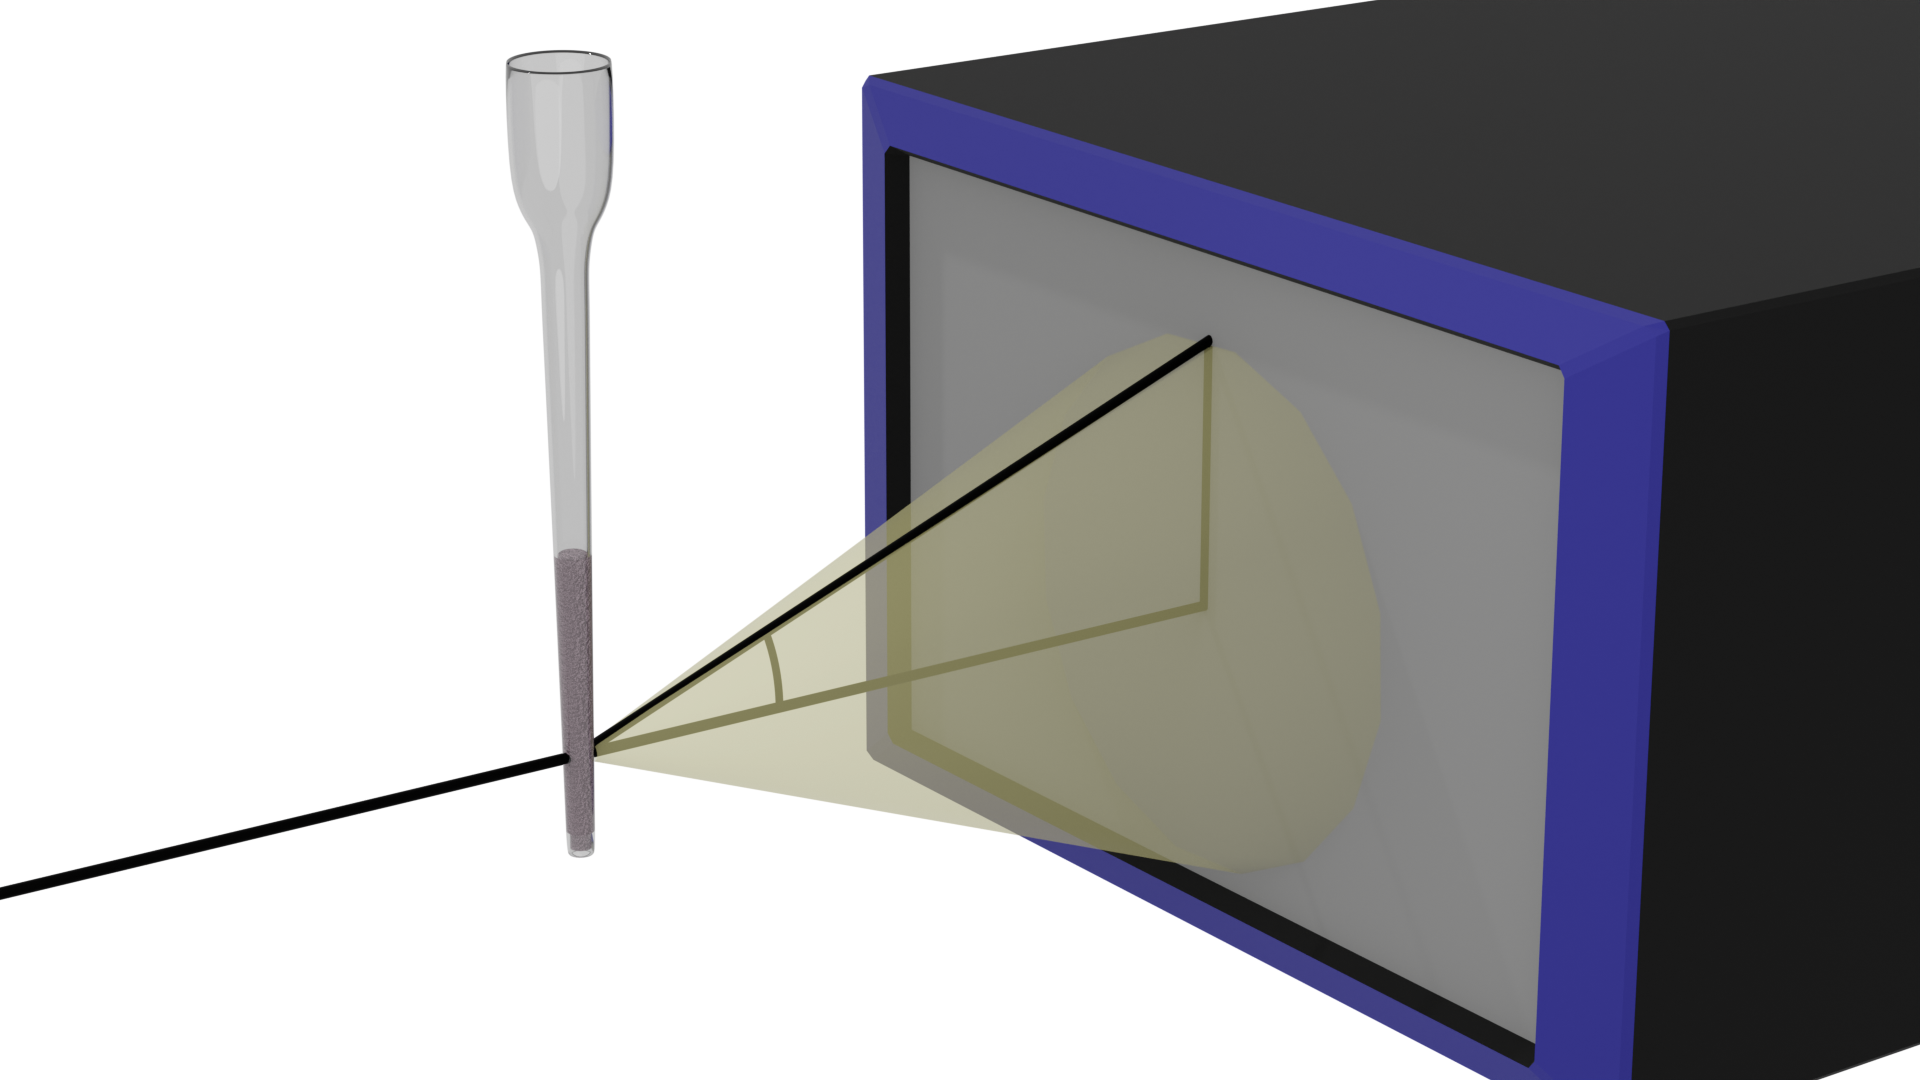
\includegraphics[width=300pt]{blender/pWAXS.png}}; \node at (4.55,2.4) {$2\theta$};
    \node at (6.9,3.3) {$r$}; \node at (5.75,2) {$d_{sd}$};
    \node at (1.2,1) {$\mathbf{k}_i$}; \node at (4.25,3) {$\mathbf{k}_s$}; \node[color=white] at (8,5.25) {area detector}; \node[anchor=east] at (2.7,5) {capillary};
    \draw[<-,thick] (3,2) -- ++ (-1,0) node[anchor=east] {sample};
    \draw (0,4) coordinate(o);
    \draw[->,>=latex] (o) --++ (0,.5) node[anchor=south]{$z$};
    \draw[->,>=latex] (o) --++ (.4,.15) node[anchor=west]{$y$};
    \draw[->,>=latex] (o) --++ (.15,-.25) node[anchor=north]{$x$};
\end{tikzpicture}
    
\end{document}